\section{CNN vs ViT}
\begin{frame}{}
    \LARGE Vision Transformers: \textbf{CNN vs ViT}
\end{frame}

\begin{frame}{CNN vs ViT}
\only<1>{
\begin{figure}
\centering
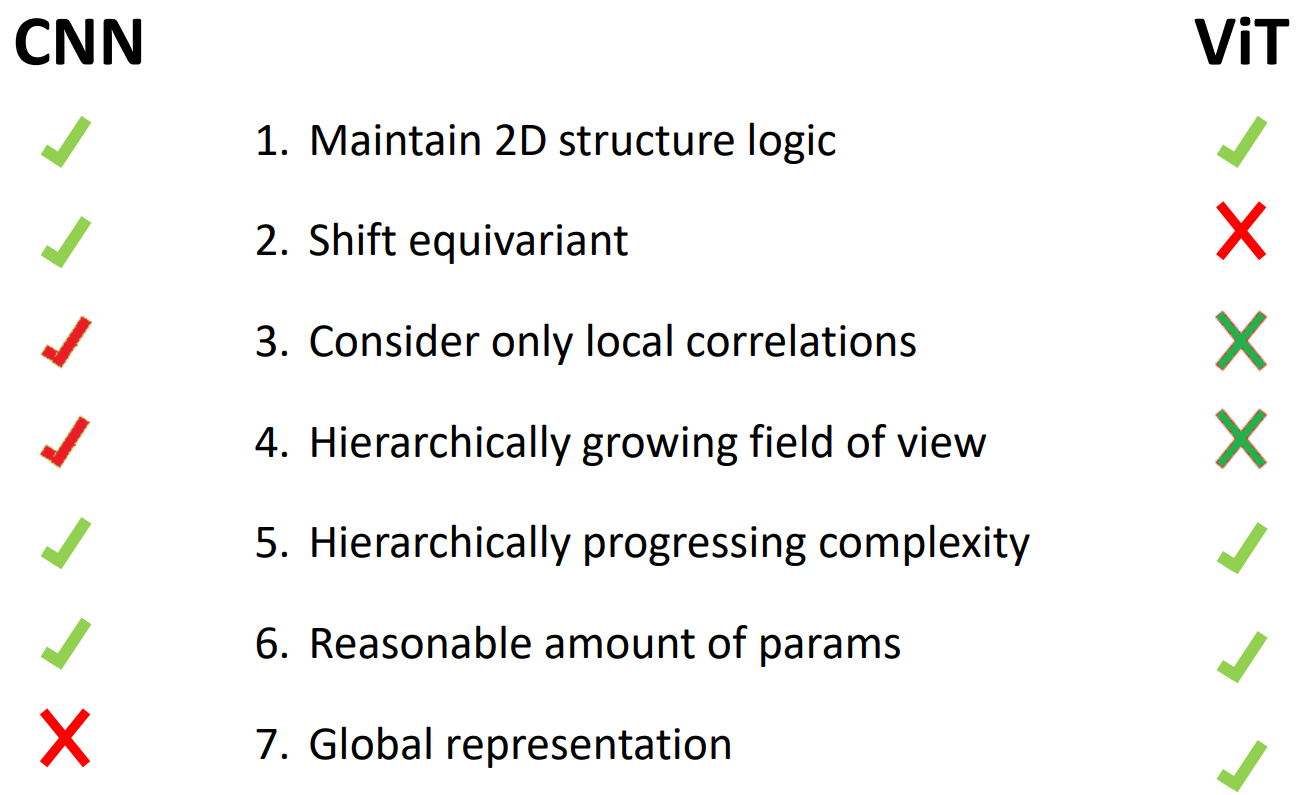
\includegraphics[width=1.0\textwidth,height=0.82\textheight,keepaspectratio]{images/advanced-cv/vit_10.png}
\caption*{\tiny Source: WAIC DL4CV, ``From Sequences to ViT'' (S. Bagon), slide 30}
\end{figure}
}

\only<2>{
\begin{figure}
\centering
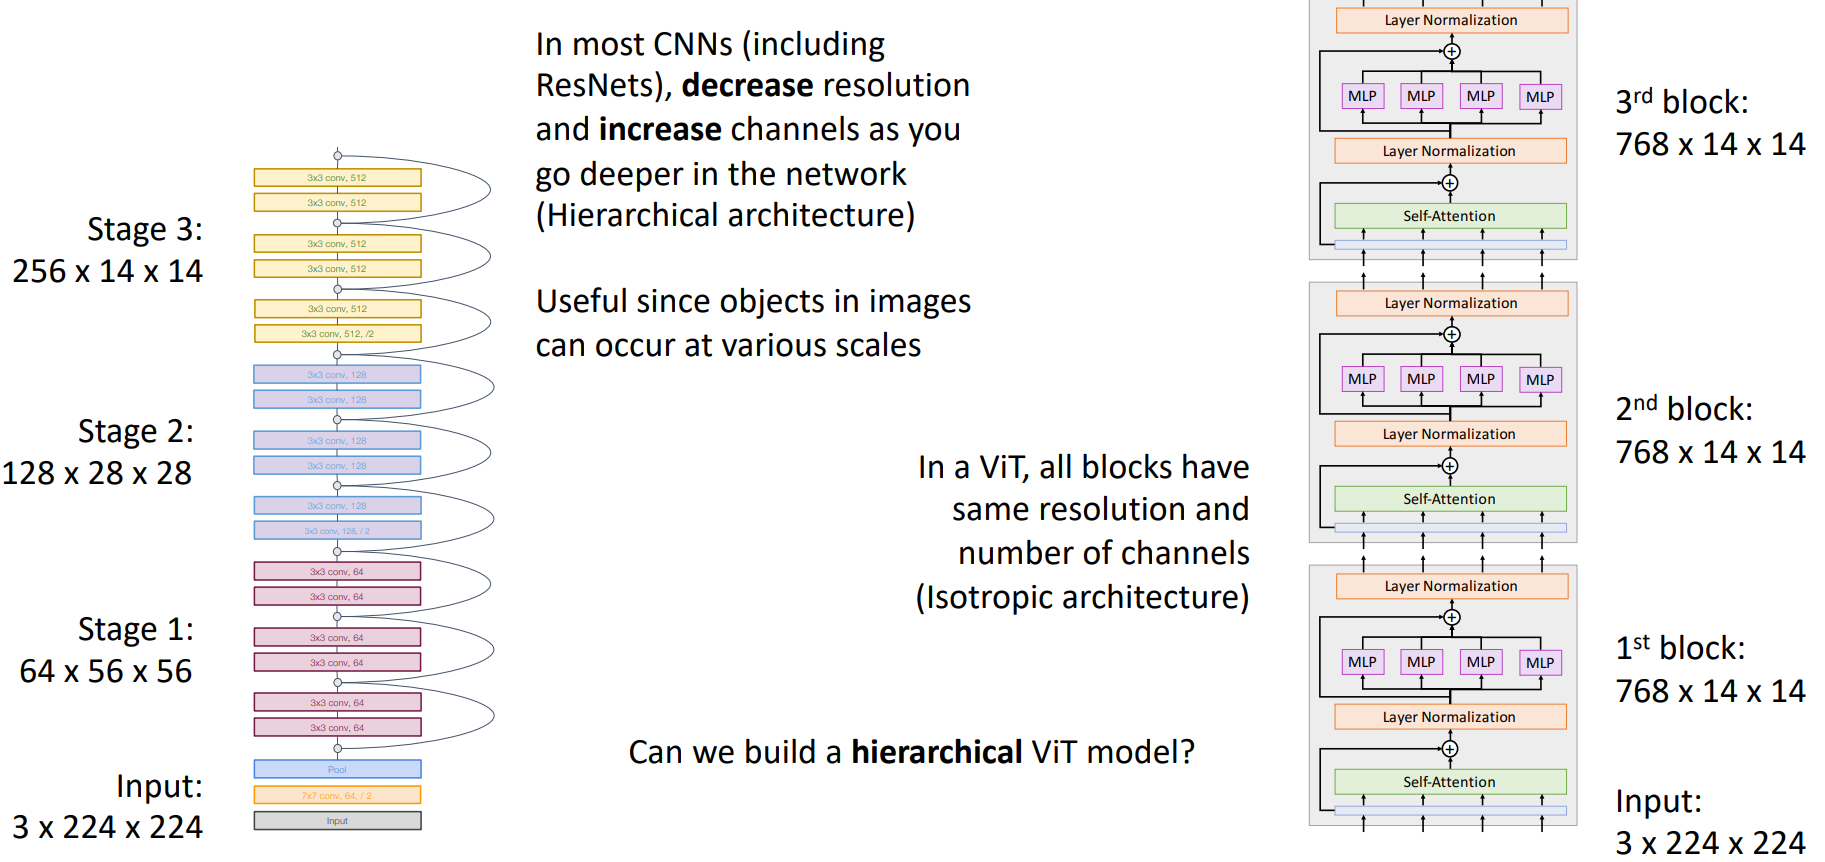
\includegraphics[width=1.0\textwidth,height=0.82\textheight,keepaspectratio]{images/advanced-cv/vit_11.png}
\caption*{\tiny Source: UMich EECS 498 (2022), Lecture 18: Vision Transformers, slide 91}
\end{figure}
}
\end{frame}

\begin{frame}{CNNs vs Vision Transformers: Key Differences}
\begin{table}[]
\centering
\begin{tabular}{|l|c|c|}
\hline
\textbf{Feature} & \textbf{CNNs} & \textbf{Vision Transformers} \\
\hline
Locality & Strong inductive bias & Weak (learns from data) \\
Parameter sharing & Yes & Yes \\
Global context & Limited & Native support \\
Training data & Efficient on small data & Needs large data or pretraining \\
Flexibility & Less modular & More modular \\
\hline
\end{tabular}
\end{table}
\end{frame}